% This file should be replaced with your file with an appendices (headings below are examples only)

% Placing of table of contents of the memory media here should be consulted with a supervisor
\chapter{Contents of the included storage media}
\dirtree{%
.1 /.
.2 src ---- source codes.
.3 enoss ---- ENOSS repository.
.4 benchmark ---- benchmark results.
.5 expr1 ---- benchmark resuls for experiment 1.
.5 expr2 ---- benchmark resuls for experiment 2.
.5 expr3 ---- benchmark resuls for experiment 3.
.5 k8s ---- k8s sources used for benchmarking.
.4 demo ---- OpenStack Swift demo with enabled ENOSS.
.4 enoss ---- ENOSS source codes.
.5 destinations ---- destination handlers.
.5 payloads ---- payload handlers.
.5 filter\_rules ---- filter rule handlers.
.4 etc/swift/enoss ---- configuration.
.4 test ---- ENOSS tests.
.5 functional.
.5 unit.
.3 mqtt-to-beanstalkd ---- source codes for MinIO proxy from MQTT to Beanstalkd
}

\chapter{Repository and Usage Guide}
ENOSS repository is publicly avaliable at the Github {\url{https://github.com/xvasil03/enoss}}.

\textbf{Demo} - OpenStack Swift demo with enabled and configured ENOSS to publish notifications to Beanstalkd queue is located in \texttt{enoss/demo}. Demo can be runned using script \texttt{run\_docker\_demo.sh}, which will create and run docker image. Demo will at start run all unit and functional ENOSS tests. Messages sent to beanstalkd queue will be shown to stdout of created docker container (messages will be in docker logs).

\textbf{Mqtt-to-Beanstalkd Demo}
\begin{enumerate}
    \item \begin{verbatim} cd mqtt-to-beanstalkd\end{verbatim}
    \item \begin{verbatim} docker-compose build\end{verbatim}
    \item \begin{verbatim} docker-compose run\end{verbatim}
\end{enumerate}

\textbf{Build} - output located in \texttt{enoss/dist}
\begin{enumerate}
    \item \begin{verbatim} cd enoss\end{verbatim}
    \item \begin{verbatim} python3 setup.py sdist bdsit_wheel\end{verbatim}
\end{enumerate}

\textbf{Instalation - OpenStack Swift (Python 2)}
\begin{enumerate}
    \item \begin{verbatim} pip install enoss/dist/*whl\end{verbatim}
    \item \begin{verbatim} pip install -r enoss/requirements-py2.txt\end{verbatim}
    \item \begin{verbatim} store configurations files from enoss/etc (needed for ENOSS configuration)\end{verbatim}
\end{enumerate}

\textbf{Instalation - OpenStack Swift (Python 3)}
\begin{enumerate}
    \item \begin{verbatim} pip3 install enoss/\end{verbatim}
    \item \begin{verbatim} pip3 install -r enoss/requirements.txt\end{verbatim}
    \item \begin{verbatim} store configurations files from enoss/etc (needed for ENOSS configuration)\end{verbatim}
\end{enumerate}

\textbf{Adding ENOSS to Proxy server} - \texttt{enoss/etc} contains example of ENOSS configuration for OpenStack Swift.
\begin{enumerate}
    \item \begin{verbatim} Add enoss to proxy server pipeline (behind s3api and bulk middleware)
    in proxy-server.conf./\end{verbatim}
    \item \begin{verbatim} Configure ENOSS using section [filter:enoss] in proxy-server.conf.\end{verbatim}
    \item \begin{verbatim} Configure destinations configuration using file speicified in
    destinations_conf_path. \end{verbatim}
    \item \begin{verbatim} Restart proxy server (swift-init proxy restart).\end{verbatim}
\end{enumerate}

\textbf{Adding ENOSS to Proxy server}
\begin{enumerate}
    \item \begin{verbatim} Add enoss to proxy server pipeline (behind s3api and bulk middleware)
    in proxy-server.conf.\end{verbatim}
    \item \begin{verbatim} Configure ENOSS using section [filter:enoss] in oio-proxy-server.conf.\end{verbatim}
    \item \begin{verbatim} Configure destinations configuration using file speicified in
    destinations_conf_path. \end{verbatim}
    \item \begin{verbatim} Restart oio-proxy server.\end{verbatim}
\end{enumerate}

\textbf{Enabling notification configuration on a container}
\begin{enumerate}
    \item \begin{verbatim} Store notification configuration using ENOSS POST API.\end{verbatim}
    \item \begin{verbatim} Check if test event was sent to specified destination
    in stored configuration.\end{verbatim}
\end{enumerate}



%\chapter{Configuration file}

%\chapter{Scheme of RelaxNG configuration file}

\chapter{Excel@FIT Article}
Article with title: "ENOSS - Event Notifications in OpenStack Swift" published and presented on April 30, 2022 at student conference Excel@FIT2022.
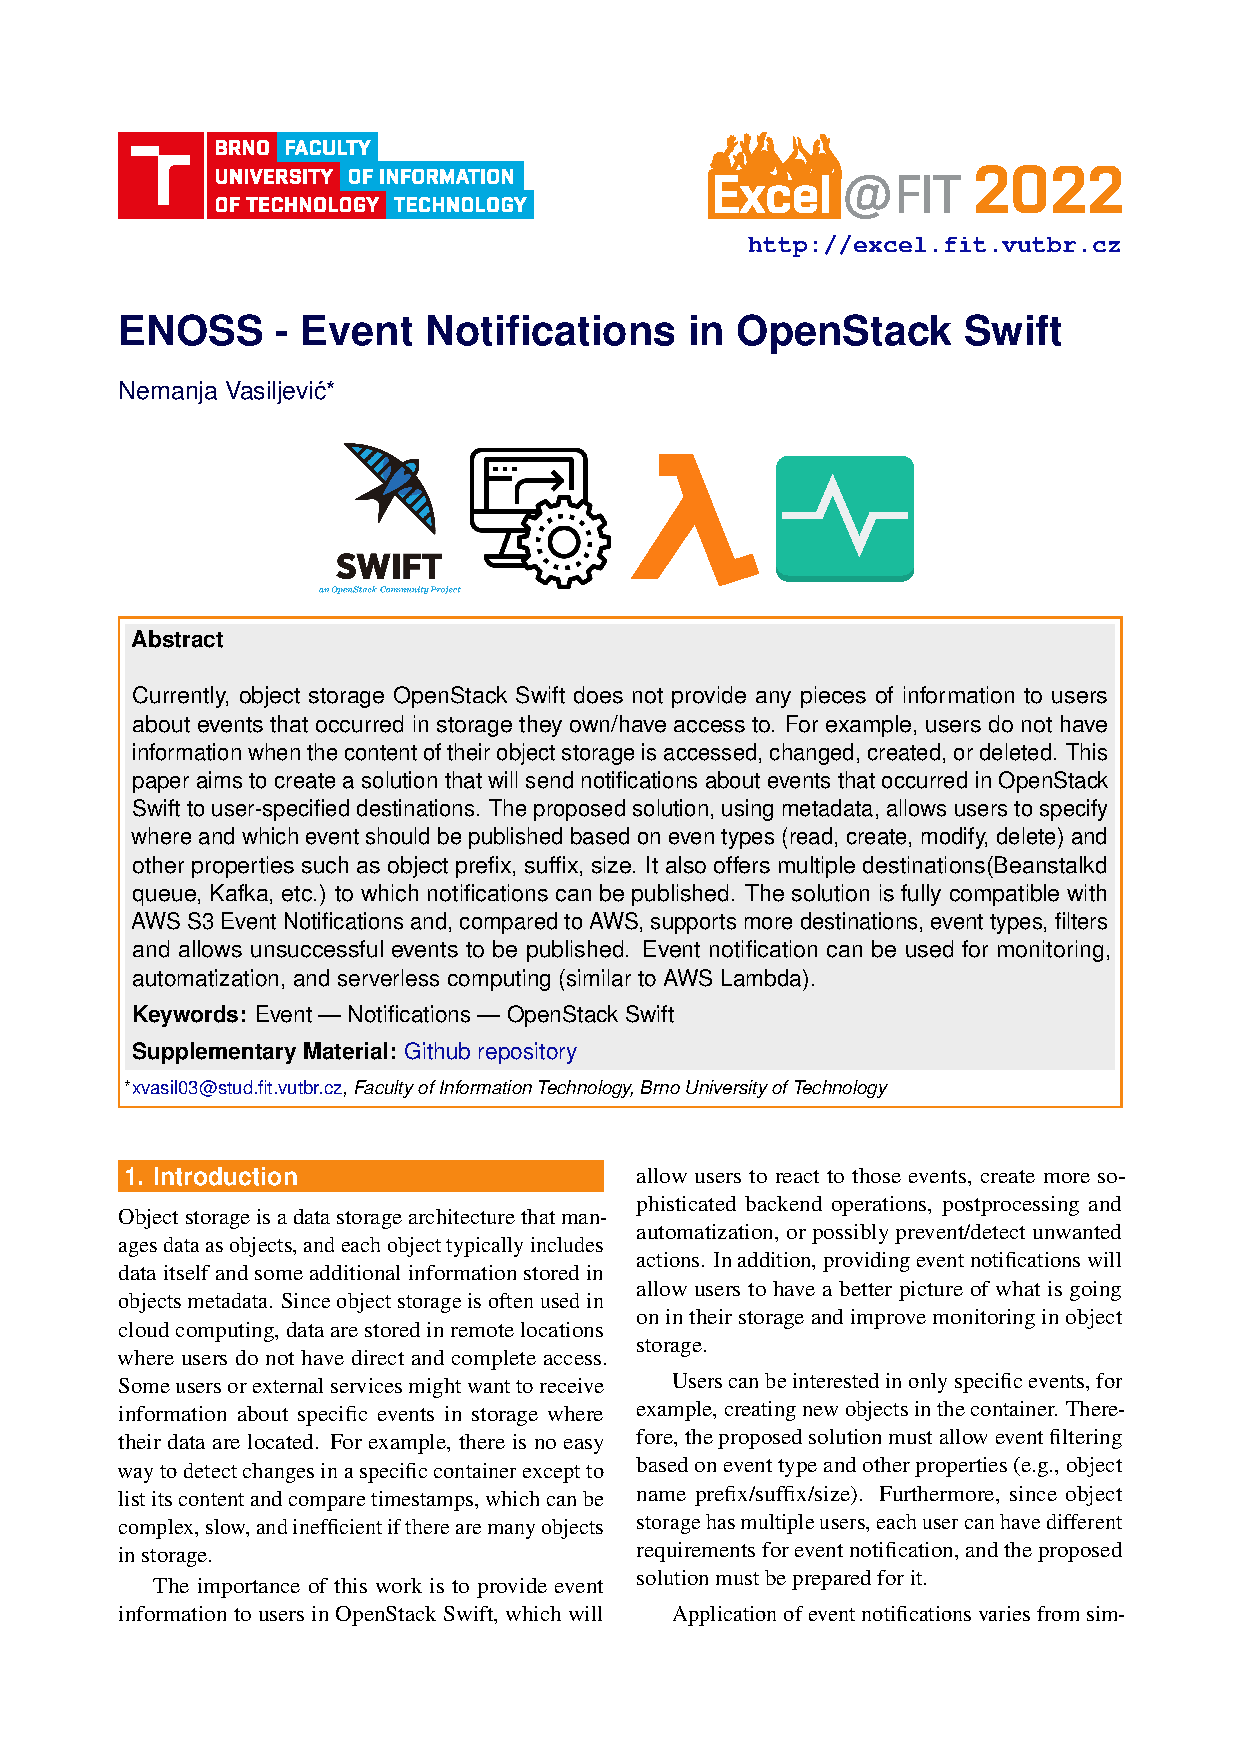
\includepdf[pages=-]{excel-paper.pdf}
